\chapter{Fundamentação Teórica}
\label{cap:conceituacao}

O desempenho de um aplicação paralela depende de uma multitude de fatores como \textit{hardware}, técnicas de otimização, topologia, arquitetura utilizada, políticas tomadas e comunicação. Na Seção~\ref{sec:parellel} são abordadas questões relacionadas a computação paralela, incluindo algumas de suas características e alguns de seus limites. A Seção~\ref{sec:topologia} aborda topologias de sistemas paralelos, suas características, seu impacto na aplicação e algumas abstrações de topologia disponíveis. Na Seção~\ref{sec:lb} é tratado o que é um balanceador de carga, que problemas estes buscam resolver e os benefícios de um balanceador ciente de topologia.


\section{Computação Paralela}
\label{sec:parellel}

Uma aplicação paralela realiza computação de maneira concorrente, utilizando os recursos de processamento disponíveis simultaneamente para a realização destas tarefas. O ganho de desempenho ao se realizar tarefas simultaneamente é pago com uma complexidade maior de \textit{hardware}, arquiteturas e com a necessidade de sincronização, garantias de exclusão, trocas de mensagem e outras técnicas de programação e compilação~\cite{david-encyclopedia}.

O fim da lei de Moore~\cite{patterson} e o limite da barreira de potência tornou a redução dos transistores e o aumento na frequência dos processadores insuficiente, abrindo um espaço para os ganhos de arquiteturas paralelas~\cite{tanenbaum:operational_systems}. Em ambientes de múltiplos núcleos se utiliza um número maior de núcleos menos poderosos, em busca de eficiência através de um paralelismo maior e de um consumo de energia mais baixo~\cite{snir-encyclopedia}. Estes sistemas são facilmente escalados através da inclusão de mais núcleos e extensão da rede, mas agregam uma série de complexidades para o desenvolvimento devido a outros fatores, como sincronização, dependência e distribuição de dados, balanceamento de carga e custos de comunicação entre os núcleos~\cite{pilla-thesis}.

A relação entre a aceleração de uma aplicação $(\textbf{S})$ com o número de núcleos utilizados ($n$) e sua parcela paralelizável ($s$) é expressa pelo argumento de Amdahl na Equação~\ref{eq:amdahl}~\cite{amdahl}. É importante constatar que são desconsiderados detalhes como os custos de acesso a memória, envio de mensagens, geração de \textit{threads} e latência de interconexão. A fórmula é então utilizada como uma estimativa otimista para a aceleração e não como uma referência exata, pois o impacto exato não é simples de calcular e pode ser afetado por diversos fatores externos a execução.

\begin{equation}
\textit{\textbf{S}} = \frac{1}{(1-\textit{s}) + \frac{\textit{s}}{\textit{n}}}
\label{eq:amdahl}
\end{equation}

Na Equação~\ref{eq:amdahl}, quando $n$ tende ao infinito a equação indica um limite na aceleração de acordo com a parcela serial do programa $(1-s)$, pois esta não se beneficia da paralelização. 
Levando este limite em conta, as aplicações paralelas muitas vezes são adaptadas para que sua parte paralelizável inclua mais detalhes ou mais precisão, fazendo com que um aumento no número de PEs leve a mais informação sendo processada e não a uma aceleração~\cite{gustafson}.

\subsection{Carga e Comunicação}

O processamento a ser realizado em uma aplicação paralela é dividido em tarefas e em cargas. 
A carga representa a quantidade de processamento que uma tarefa precisa realizar em um único PE. 
Em um sistema paralelo, múltiplas tarefas são executadas simultaneamente, tendo sua carga distribuída entre os PEs do sistema. 
Um núcleo que possui uma carga maior que um limiar acima da média é considerado sobrecarregado, e um núcleo que tem menos carga que um limiar abaixo da media é considerado subcarregado. 
Esta diferença nas cargas faz com que alguns PEs não tenham trabalho para executar enquanto esperam a conclusão de tarefas nos PEs mais carregados, sub-utilizando o sistema. 
Esta situação é chamada de desbalanceamento.

\begin{figure} [b]
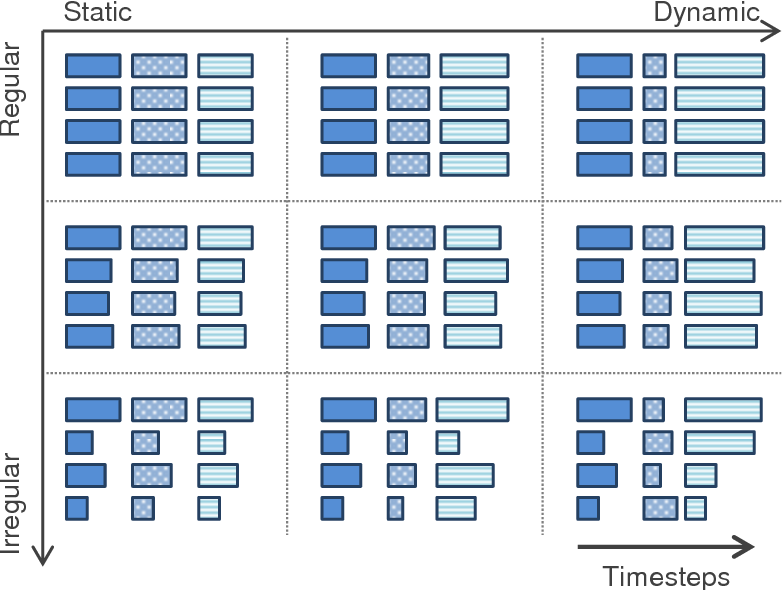
\includegraphics[width=0.62\textwidth]{load_pilla}
\centering
\caption[Diferentes graus de regularidade e dinamicidade em relação a carga de uma aplicação.]{Diferentes graus de regularidade e dinamicidade em relação a carga de uma aplicação ~\cite{pilla-thesis}.}
\label{fig:load}
\end{figure}

Em aplicações paralelas, a carga de cada tarefa e sua comunicação pode ser diferente das demais tarefas. Essas diferenças podem se manter constantes ou até mesmo variar ao longo da execução da aplicação paralela. 
Duas características refletem isso: a \textit{regularidade} e a \textit{dinamicidade}. 
A regularidade de uma aplicação reflete o quanto a carga ou a comunicação de uma tarefa difere de uma outra tarefa. Uma aplicação com carga ou comunicação regular tem cargas ou comunicação aproximadamente iguais. 
Quando a carga ou comunicação difere entre tarefas, a aplicação tem carga ou comunicação irregular, respectivamente.
A dinamicidade de uma aplicação indica o quanto a comunicação ou carga de uma tarefa muda ao longo do tempo. Quando sua carga ou comunicação não muda ao longo do tempo, é dita estática e quando muda, é dita dinâmica~\cite{pilla-thesis}.
As Figuras~\ref{fig:load} e \ref{fig:communication} apresentam a variação de regularidade e dinamicidade em relação a carga e a comunicação de uma tarefa, respectivamente. 

\begin{figure} [h]
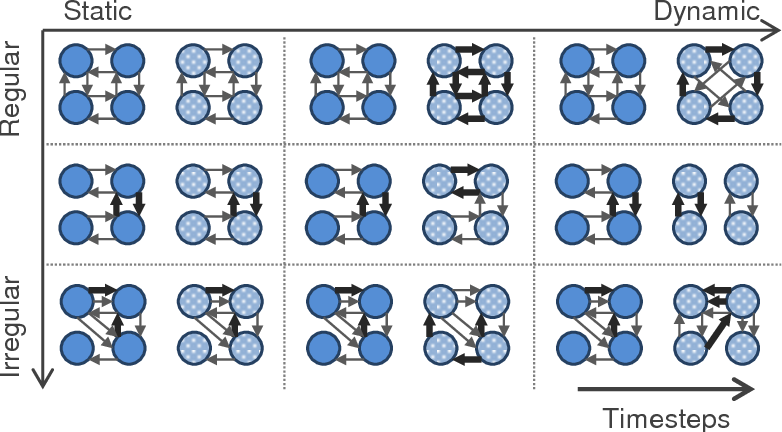
\includegraphics[width=0.67\textwidth]{comm_pilla}
\centering
\caption[Diferentes graus de regularidade e dinamicidade em relação a comunicação de uma aplicação.]{Diferentes graus de regularidade e dinamicidade em relação a comunicação de uma aplicação ~\cite{pilla-thesis}.}
\label{fig:communication}
\end{figure}

A distribuição de tarefas em um ambiente paralelo deve levar em consideração sua regularidade e dinamicidade. 
Técnicas de escalonamento, alocação de tarefas e balanceamento de carga são utilizadas para gerenciar e dispor as tarefas de maneira eficiente no sistema. 
Na Seção~\ref{sec:lb} serão abordadas algumas técnicas de balanceamento de carga.

\subsection{Computação Distribuída}

Em ambientes multiprocessados, existe algum dispositivo de memória compartilhada entre todos os PEs, o qual é organizado de forma a impedir problemas de coerência e consistência. \textit{Chips} \textit{multicore} e \textit{manycore} são exemplos de ambientes multiprocessados. 
Ambientes multiprocessados não escalam bem devido à complexidade de arquitetura e custos de produção, abrindo espaço para ambientes multicomputados. 
Em ambientes multicomputados a memória não é compartilhada entre todos os PEs e algum meio de interconexão é utilizado para realizar as trocas de informação, mas o sistema ainda é organizado de maneira similar~\cite{tanenbaum:operational_systems}.

Em um sistema distribuído, computadores com diferentes arquiteturas, organizações, locais e comportamentos podem ser interconectados em uma mesma rede e utilizados em conjunto. 
Devido à alta independência dos componentes, estes sistemas são altamente escaláveis através da adição de computadores e expansão da rede. 
A comunicação e coordenação destes sistemas se torna muito mais complexa e custosa devido ao número de componentes, precisando ser tratada com mais detalhe~\cite{tanenbaum:operational_systems}.


\section{Topologia de Rede}
\label{sec:topologia}

Sistemas paralelos utilizam redes de interconexão para efetuar a comunicação entre seus PEs. 
Estas redes têm propriedades como diâmetro, distância média, grau, latências e largura de banda que regem a comunicação dentro da rede. 
O padrão de interconexões entre PEs é chamado de topologia e esta pode assumir diversas formas como malhas, tori e \textit{fat-trees}.

As topologias de uma rede podem ser dividas em duas categorias: \textit{diretas} e \textit{indiretas}. 
Em redes diretas, os PEs são conectados diretamente  uns aos outros através de \links. Para que uma mensagem possa ser transmitida de um PE a outro, esta precisa trafegar através de vários destes \links.
O cruzamento de um \link é chamado de \hop e a distância entre um ponto a outro na rede pode ser definido pelo número de \hops realizados. 
Malhas, tori e hipercubos são exemplos de redes diretas. 
Em redes indiretas, PEs são conectados a \switches (roteadores) que roteiam as mensagens. Nenhum PE é ligado diretamente a outro PE e portanto é necessário cruzar dois ou mais \switches para alcançar outro PE. 
\Fatts e \dgfly são exemplos de redes indiretas~\cite{bhatele-encyclopedia}.

A hierarquia é um fator presente em algumas topologias indiretas, como \fatt e \dgfly, e divide esta em níveis de proximidade. 
Cada nível de hierarquia na topologia representa um agrupamento diferente da rede. 
Redes hierárquicas apresentam pontos de gargalo de tráfego entre seus níveis e requerem uma replicação de \links para que isto não se torne um problema.

Uma rede de interconexão tem duas propriedades importantes que afetam sua comunicação: \textit{simetria} e \textit{uniformidade}. 
Um nível de topologia é dito simétrico quando o tempo de comunicação de um ponto A para um ponto B é o mesmo que de B para A. Caso contrário, este é dito assimétrico. 
Um nível de topologia é uniforme quando todos os PEs neste nível tem o mesmo tempo de comunicação entre si~\cite{pilla-thesis}. 
Nesse sentido, uma rede indireta pode se tornar assimétrica devido ao roteamento de informações. 
%problema: parece estar mal formulado e estranho porque por exemplo de p1 a p3 pode ter um caminho mais longo (tori por exemplo)
%problema tem alguma utilidade falar isso?

\begin{figure} [b]
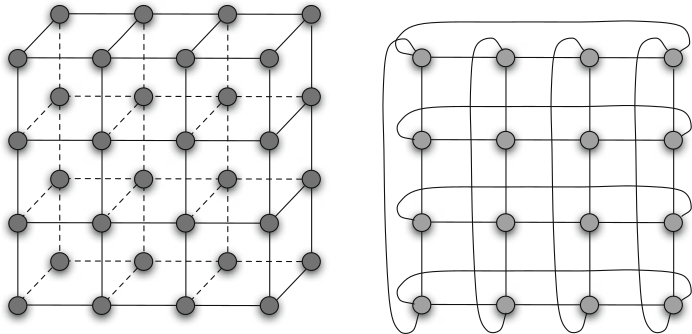
\includegraphics[width=0.5\textwidth]{mesh_torus}
\centering
\caption[Uma malha de dimensões (4,4,2) e uma torus 2D]{Uma malha de dimensões (4,4,2) a esquerda e uma torus 2D a direita~\cite{bhatele-encyclopedia}}
\label{fig:mesh_torus}
\end{figure}

Algumas métricas são utilizadas para observar o comportamento de uma rede, como o diâmetro, o número de \links, o grau e a bisseção de \links. 
O diâmetro de uma rede é definido como sendo o maior caminho dentre os caminhos mais curtos que ligam quaisquer dois nós da topologia. Usualmente, as distâncias são medidas através do número de \hops, sendo esta métrica também utilizada para determinar a maior latência dentro de uma rede. 
O número de \links apresenta a quantidade total de \links dentro da rede, uma informação usada para avaliar o custo de implantação. 
O grau de uma rede é o número de \links conectados em cada nó da rede. 
A bisseção da largura de banda representa a quantidade de \links entre duas partes da rede, partida de modo a gerar o mínimo de \links entre duas metades da rede. 
Essa métrica é utilizada para estimar o quanto de tráfego a rede suporta~\cite{david:paralel}. A seguir, são apresentadas algumas topologias abordadas neste trabalho.

\begin{figure} [t]
    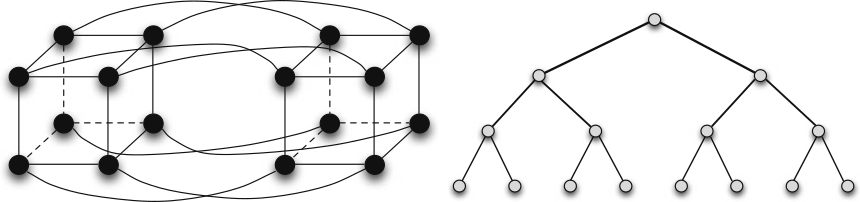
\includegraphics[width=0.7\textwidth]{hypercube_fat_tree}
    \centering
    \caption[Um hipercubo de e uma \fatt]{Uma rede direta em forma de hipercubo de 4 dimensões a direita e uma indireta em forma de \fatt binária com 4 níveis a esquerda~\cite{bhatele-encyclopedia}}
    \label{fig:cube_fat}
\end{figure}

\begin{figure} [t]
    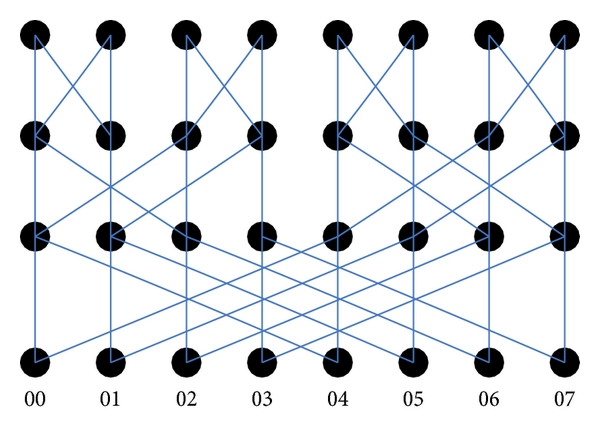
\includegraphics[width=0.4\textwidth]{bfly}
    \centering
    \caption[Uma rede \textit{Buttefly}]{Uma rede \textit{butterfly} de 3 níveis e 8 nós~\cite{Liu:bfly}}
    \label{fig:bfly}
\end{figure}

\begin{itemize}
    \item \textbf{Malha}: Uma topologia direta similar a uma matriz de múltiplas dimensões, onde cada \link só cruza uma dimensão da rede e na menor distância possível ~\cite{Solihin}.
    Malhas podem ser dispostas em diversas dimensões. A Figura~\ref{fig:mesh_torus} representa uma malha de dimensões 4, 4 e 2.
    
    \item \textbf{Torus}: Uma malha com um \link entre nodos finais de cada dimensão da rede, reduzindo o diâmetro da rede e aumentando sua bisseção. 
    Uma torus de dimensões 4 e 4 pode ser observada na Figura~\ref{fig:mesh_torus}.
    
    \item \textbf{Hipercubo}: Uma malha com 2 nodos em cada dimensão.
    Um hipercubo visa reduzir a distancia máxima da rede. 
    A Figura~\ref{fig:cube_fat} mostra um exemplo de hipercubo.
    
    \item \textbf{\Fatt}: Uma topologia de rede indireta em forma de árvore, onde \links em níveis mais altos possuem mais largura de banda. 
    Esta topologia é encontrada como topologia interna de máquinas. 
    Uma \fatt é representada na Figura~\ref{fig:cube_fat}.
    
    \item \textbf{\textit{Butterfly}}: Uma topologia indireta que visa escalabilidade e redução de distâncias através da replicabilidade de \links e de roteadores.
    É utilizada para gerar uma bisseção de banda elevada dentro de uma rede.
    Sua desvantagem é o grande número de \links, o qual é muito superior ao de outras topologias~\cite{david:paralel}.
    
    \item \textbf{\Dgfly}: Uma topologia indireta que cria agrupamentos de roteadores em grupos distintos, visando reduzir o número de \links da rede para reduzir seu custo.
   
    
    \item \textbf{\textit{Slim Fly}}: Uma topologia indireta similar a \dgfly mas otimizada matematicamente, reduzindo o custo e energia gasta enquanto aumenta a resiliência da rede em relação à falha de \links~\cite{slimfly}.
\end{itemize}

\setlength{\tabcolsep}{0.5em}
\begin{table}[t]
    \centering
    \begin{tabular}{c l}
        \toprule
        \textbf{Símbolo} &    \textbf{Descrição}  \\ \midrule
        $d$ & Número de dimensões da topologia.  \\ %\hline
        $k$ & Número de nós por dimensão da topologia.  \\ %\hline
        $p$ & Número de nós totais da topologia.  \\ %\hline
        $f$ & Valor de \textit{fanout} da árvore.  \\ %\hline
        $h$ & Número de \links remotos por roteador \\ %\hline
        $r$ & Número de roteadores por grupo \\ \bottomrule
    \end{tabular}
    \caption[Símbolos utilizados na Tabela~\ref{tab:topo_comparison}]{Símbolos utilizados na Tabela~\ref{tab:topo_comparison}.}
    \label{tab:topo_symbols}
\end{table}

\setlength{\tabcolsep}{0.5em}
\renewcommand{\arraystretch}{1.1}
\begin{table}[t]
    \centering
    \begin{tabular}{l c c c c}
        \toprule
        \textbf{Topologia} &    \textbf{Diâmetro} &  \textbf{Bisseção} &   \textbf{\Links} &     \textbf{Grau} \\ \midrule
        Malha 2-D & $2\sqrt{p}-1$ & $\sqrt{p}$ &   $2\sqrt{p} \times (\sqrt{p}-1)$ &    $2d$  \\ %\hline
        Malha K-D & $dk-1$ & $k^{d-1}$ &   $dk^{d-1} \times (k-1)$ &    $2d$  \\ %\hline
        Tori  & $\frac{dk}{2}-1$ & $k^d$ & $dk^d$ &  $2d$  \\ %\hline
        Hipercubo &  $\log_2 p$ & $\frac{p}{2}$ &  $log_2 p \times \frac{p}{2}$  &  $\log_2 p$  \\ %\hline
        \Fatt &  $2 \times \log_f p$ & $\frac{p}{2}$ & $f(p-1)$ &  $f + 1$  \\ %\hline
        \textit{Butterfly} & $\log_2 p$ & $\frac{p}{2}$ &  $2p \times \log_2 p$ &  $4$  \\ %\hline
        \Dgfly & $3$  & $h((r+2)^2/4) $  &  $ r\times(r-1) +rh  $ & $r + h$ \\ 
        \textit{Slim Fly} & $2$  & - &  $2\times r\times(r-1)$ & $r + h$ \\\bottomrule
    \end{tabular}
    \caption[Diâmetro, bisseção de \links, número \links e grau das topologias de Malha, Tori, Hipercubo, \Fatt, \textit{Butterfly}, \Dgfly e \textit{Slim Fly}.]{Diâmetro, bisseção de \links, número de \links e grau das topologias Malha, Tori, Hipercubo, \Fatt, \textit{Butterfly}, \Dgfly~\cite{li:dgfly} e \textit{Slim Fly}. Os símbolos utilizados são apresentados na Tabela~\ref{tab:topo_symbols}. Adaptado de ~\cite{Solihin}. A topologia \textit{Slim Fly} não apresenta uma fórmula de bisseção, pois ela é calculada aproximadamente utilizando um particionador. Sua bisseção é maior que uma \dgfly mas menor que de um hipercubo~\cite{slimfly}.}
    \label{tab:topo_comparison}
\end{table}

A Tabela~\ref{tab:topo_comparison} apresenta algumas topologias e suas características principais: diâmetro, bisseção, \links e grau. Os símbolos utilizados são descritos na Tabela~\ref{tab:topo_symbols}.
É importante ressaltar que $p = dk$ nas topologias de Malha ou Tori.
Na Tabela~\ref{tab:topo_example} são comparadas topologias com $2^{16}$ nós.
A topologia \dgfly se destaca, pois tem \links com latências diferentes e custos de implementação diferentes, fazendo com que métricas baseadas em \hops e número de \links não reflitam a distância e o desempenho da rede.


\setlength{\tabcolsep}{0.5em}
\begin{table}[t]
    \centering
    \begin{tabular}{l c c c c}
        \toprule
        \textbf{Topologia} &    \textbf{Diâmetro} &  \textbf{Bisseção} &   \textbf{\Links} &     \textbf{Grau} \\ \midrule
        Malha 4D & $63$ & $4096$ & $245760$ &  $8$  \\ %\hline
        Tori 4D & $31$ & $65536$ & $262143$ &  $8$  \\ %\hline
        Hipercubo &  $16$ & $32768$ &  $524288$  &  $16$  \\ %\hline
        \Fatt &  $16$ & $32768$ & $262143$ &  5  \\ %\hline
        \textit{Butterfly} & $16$ & $32768$ &  $2097152$ &  $4$  \\ %\hline
        \Dgfly & $3$  & $4225$  &  $ 16896 $ & $129$ \\
        \textit{Slim Fly} & $3$  & $4225$  &  $ 16896 $ & $129$ \\ \bottomrule
    \end{tabular}
    \caption[Diâmetro, bisseção de banda, número de \links e grau das topologias com 64000 nodos.]{Diâmetro, bisseção de banda, número de \links e grau das topologias de Malha 4D, Tori 4D, Hipercubo, \Fatt de \textit{fanout} 4, \textit{Butterfly} e \Dgfly, todas com $2^{16}$ (65536) nodos.}
    \label{tab:topo_example}
\end{table}


Conforme cresce o número de PEs de um sistema, o fluxo de informação na rede aumenta e mais recursos de rede (\links e \switches) são compartilhados e disputados pelos PEs.
Este compartilhamento pode levar a um problema chamado de contenção, onde a latência da rede aumenta devido a saturação dos \links.
Um mapeamento de tarefas ciente de topologia de rede pode reduzir o compartilhamento de recursos de rede e portanto melhorar o desempenho da aplicação~\cite{bhatele-encyclopedia}.

\begin{figure} [h]
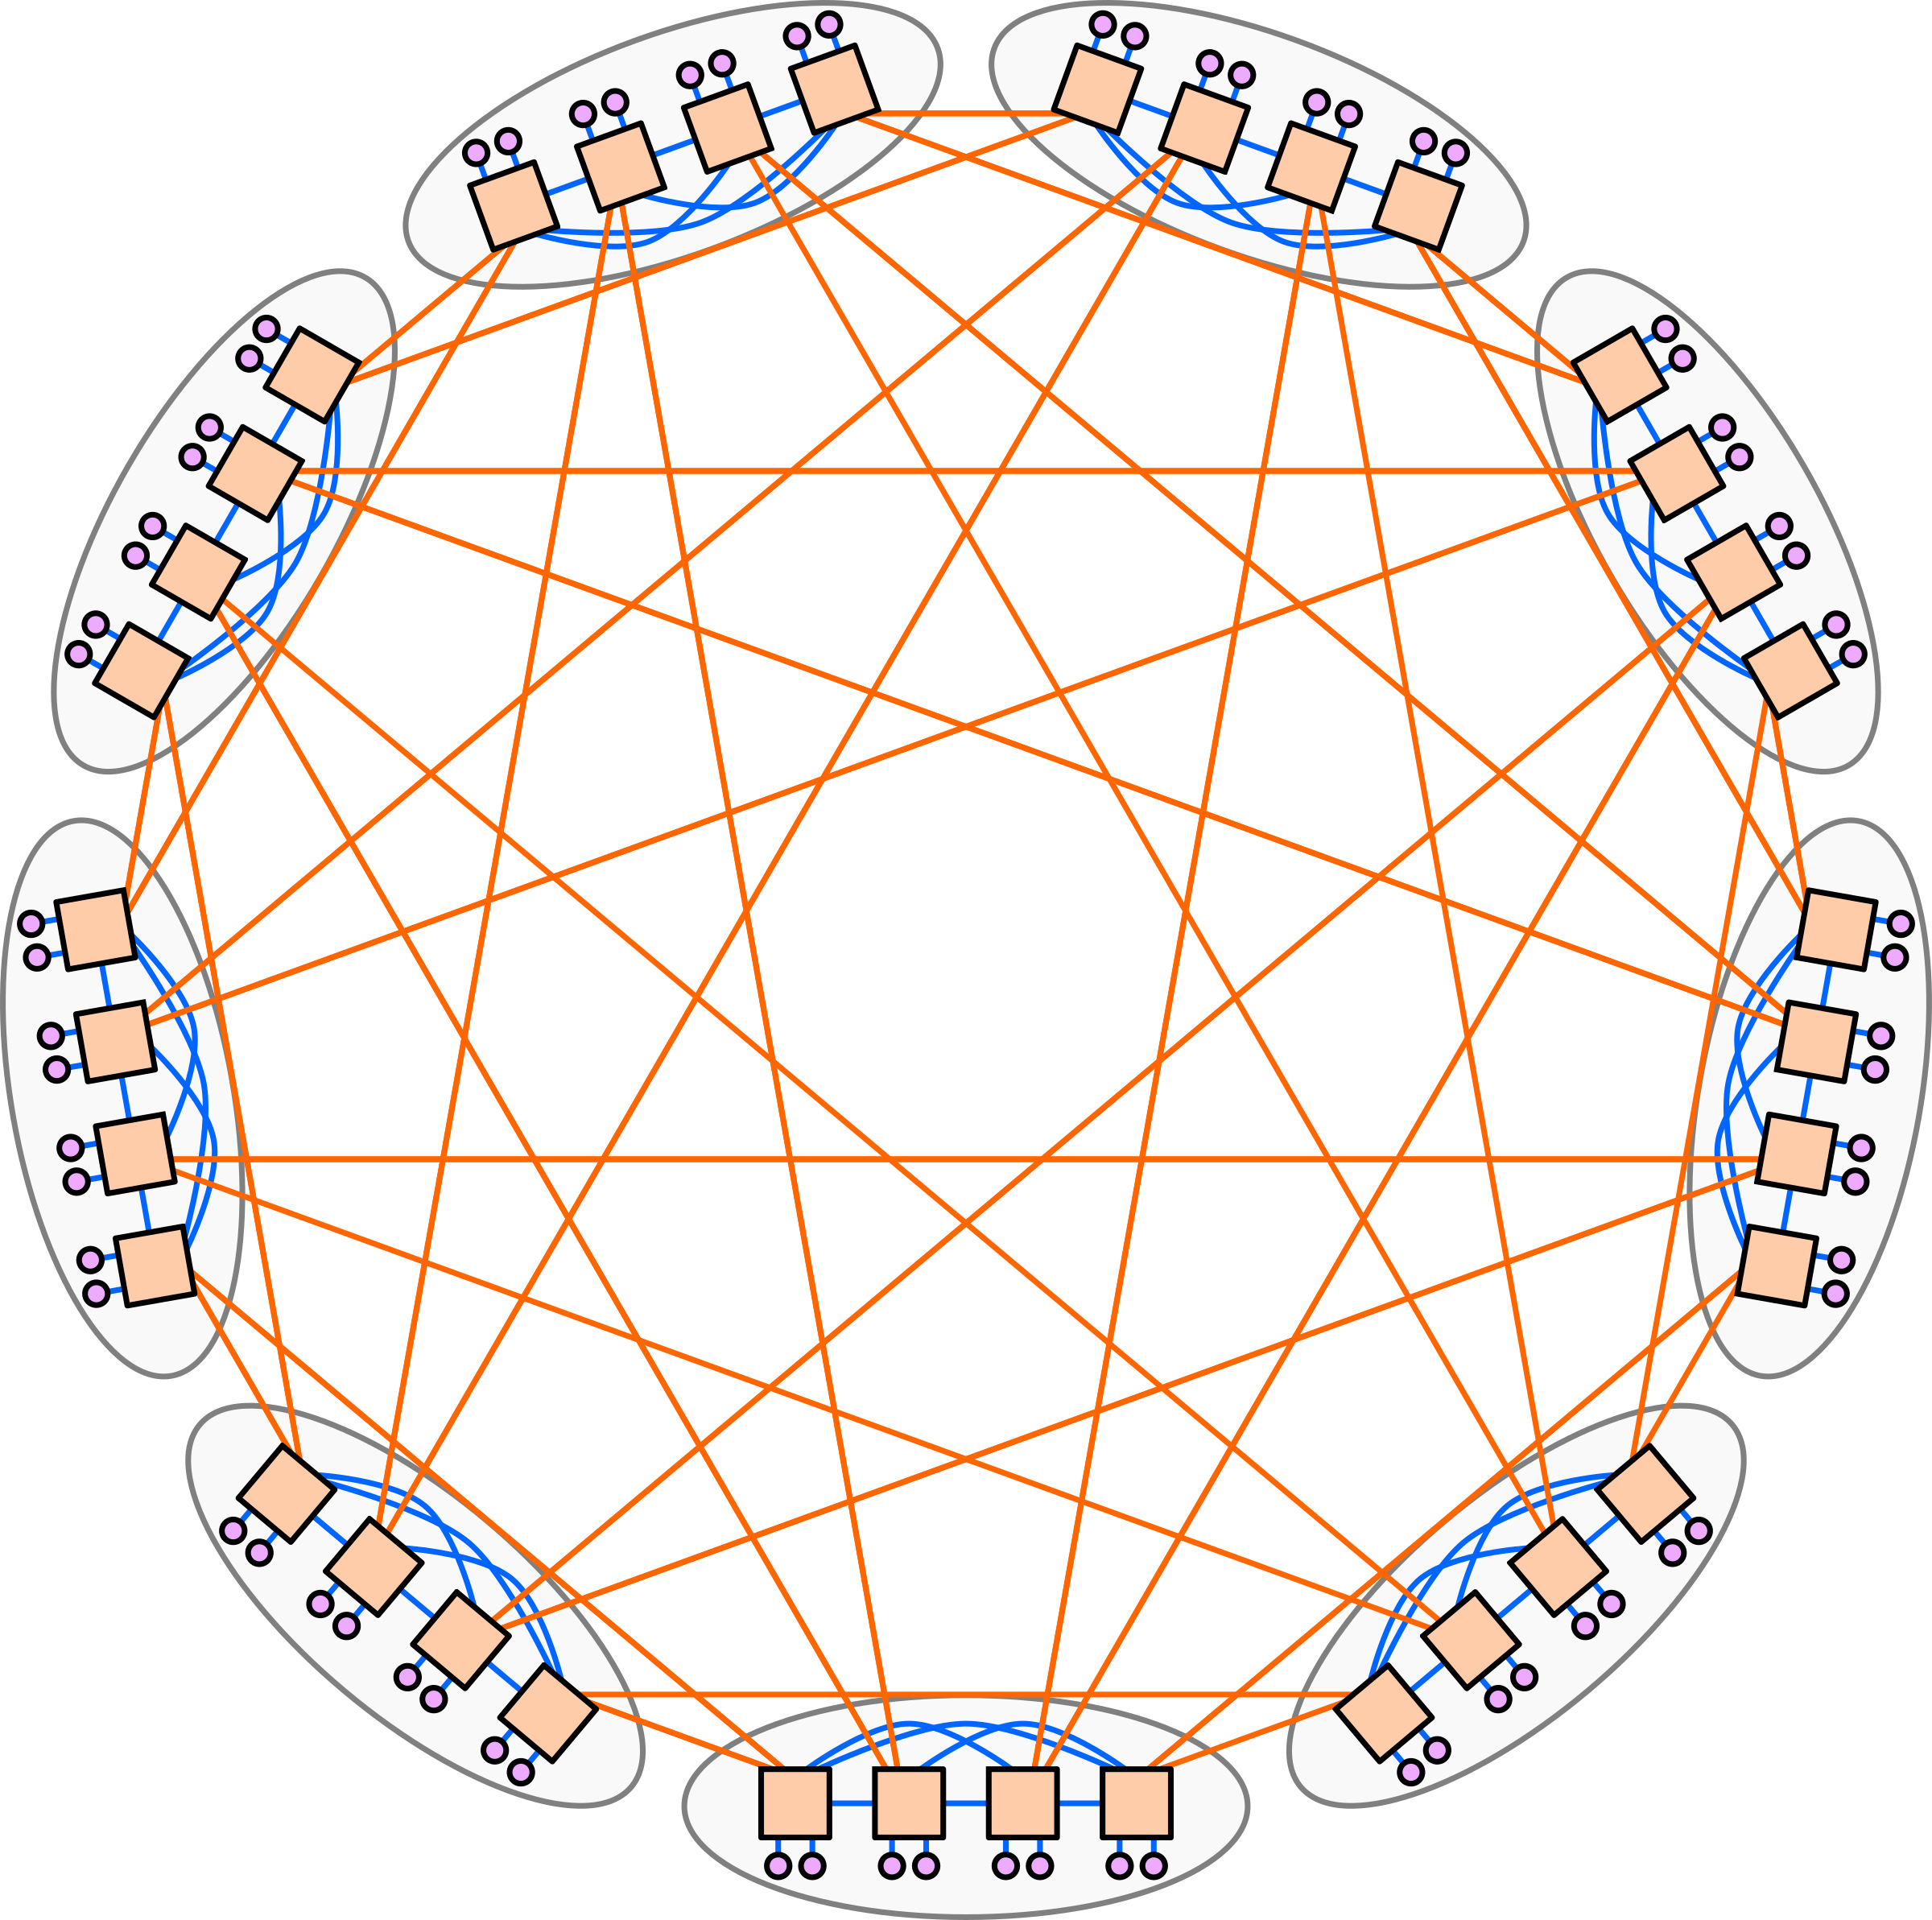
\includegraphics[width=0.6\textwidth]{dragonfly}
\centering
\caption[Um exemplo de rede \dgfly.]{Um exemplo de rede \dgfly. Roteadores e \links globais em laranja, nós em vermelho e \links locais em azul. Fonte: Openclipart, \url{https://openclipart.org/detail/291507/dragonfly-network-topology}, acessado em 08 nov. 2018}
\label{fig:dgfly}
\end{figure}

Topologias de rede podem ter agrupamentos de máquinas interligados com \links de maior latência ou menor capacidade, como, por exemplo, a \dgfly da Figura \ref{fig:dgfly}.
A contenção e a alocação de tarefas neste tipo de rede afeta severamente seu desempenho.
Nestas redes, uma política adequada de roteamento, de alocação de tarefas, de migração de tarefas e de carga de trabalho paralela é crucial~\cite{dragonfly}.
Roteamento dinâmico e adaptativo é um exemplo de política geralmente acoplado a redes deste tipo, para que decisões de roteamento levem em consideração a atual contenção da rede. 
Com isso, caminhos menos sobrecarregados são tomados, distribuindo melhor a carga da rede e evitando problemas graves de contenção~\cite{kim:2008}. 
Balanceamento de carga ciente de topologia se torna um fator ainda mais relevante para este tipo de rede.

%\begin{figure} [h]
%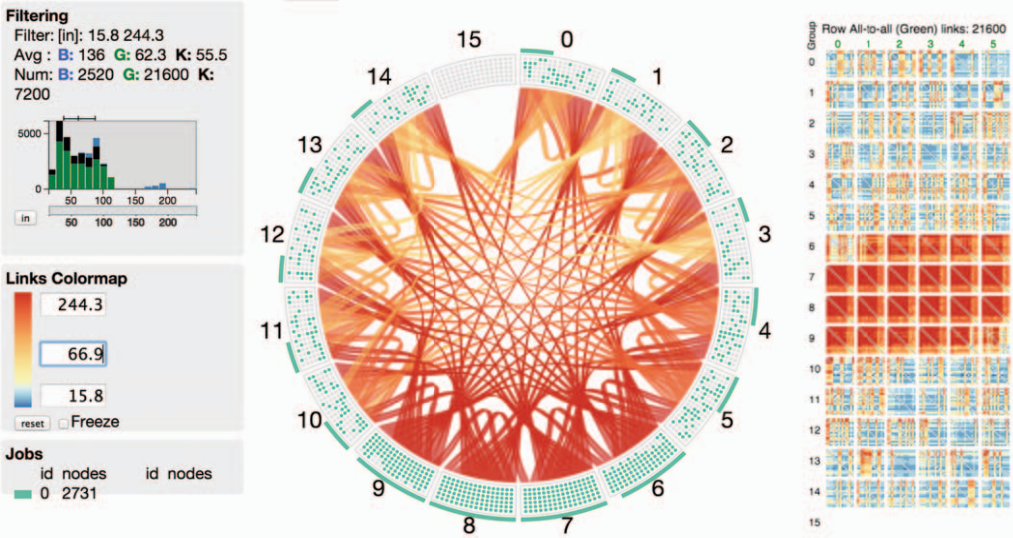
\includegraphics[width=0.8\textwidth]{dgfly_bhat}
%\centering
%\caption[Exemplo de rede \dgfly de três níveis com 64000 nós em execução, onde 2731 estão alocados para uma tarefa]{Exemplo de rede \dgfly de três níveis com 64000 nós em execução, onde 2731 estão alocados para uma tarefa. \Links globais apresentados no meio e links locais na matriz a direita. Quanto mais avermelhado, mais tráfego na rede~\cite{dragonfly}.}
%\label{fig:dgfly_bhat}
%\end{figure}

\subsection{Abstrações de Topologia}
\label{sec:abstrações}

Nesta seção são abordados dois trabalhos que abstraem informações de topologia para seu uso em aplicações: O \textit{Portable Hardware Locality} (\hwloc) \cite{broquedis:hwloc} e o \textit{Portable Network Locality}  (\netloc) \cite{Goglin:netloc}.

\Hwloc é um \textit{software} que provê uma abstração da hierarquia das arquiteturas de máquinas, dispondo uma série de informações de \textit{cache}, núcleos, \textit{multithreading}, \textit{sockets} e dispositivos de entrada e saída~\cite{broquedis:hwloc}.
Seu objetivo é facilitar o acesso de informações complexas das arquiteturas atuais, de maneira uniforme e portável para aplicações.
Em sistemas Unix, por exemplo, as informações coletadas por \hwloc estão em diversos arquivos espalhados pelo sistema. Portanto, diversas leituras de dados em disco são necessárias para adquirir estas informações.
Em questão de topologia, o \hwloc trabalha somente em um ambiente multiprocessado, em uma única máquina, não oferecendo suporte em relação a topologia de um ambiente multicomputado ou distribuído.

\Netloc~é um projeto de \textit{software} acoplado ao \hwloc que provê uma abstração da topologia de rede.
Assim como o \hwloc, o \textit{software} é usado para encontrar informações completas da topologia, ainda não descobertas, e disponibilizá-las para o usuário.
O trabalho do \netloc é voltado para métodos de descobrimento e representação da topologia de rede, unindo estas informações com as informações de máquina do \hwloc~\cite{Goglin:netloc}.

O projeto \netloc ainda está em desenvolvimento e ainda não possui representação de distância ou latência entre áreas distintas da rede.
Além disso, sua preocupação é de fornecer todas as informações que conseguir sobre a topologia utilizada de maneira dinâmica para considerar alterações na rede devido a falhas e expansões~\cite{Goglin:netloc}.
A quantidade e complexidade destas informações aumentam a ocupação de memória e o tempo de inicialização da abstração, adicionando um custo indesejado.

\section{Balanceamento de Carga}
\label{sec:lb}

Balanceamento de carga é uma técnica que realiza distribuição de cargas de computação e comunicação em um sistema de maneira que nenhum processador seja sobrecarregado e que reduza custos de comunicação~\cite{Becker}. 
Tendo em vista uma aplicação dinâmica, a distribuição de carga e comunicação se altera ao longo da aplicação, sendo necessário realizar um balanceamento de carga periodicamente para mitigar o desbalanceamento. 

Encontrar um mapeamento ótimo para uma aplicação paralela executada em múltiplas máquinas idênticas é um problema NP-\textit{hard}~\cite{leung}. 
Como o objetivo de balancear é aumentar o desempenho, utilizam-se heurísticas para realizar um balanceamento sub-ótimo, já que um mapeamento ótimo iria demorar a ponto de degradar o tempo da aplicação~\cite{pilla-thesis}.

Um balanceador de carga (\textit{Load Balancer} ou LB) pode administrar informações sobre a distribuição de carga e comunicação de três maneiras: \textit{centralizada}, \textit{distribuída} e \textit{hierárquica}.
Um LB centralizado administra a informação do sistema como um todo, podendo realizar decisões mais completas, mas criando um gargalo de informações. 
Um LB distribuído é o outro extremo pois observa somente informações locais, tendo um processo de balanceamento mais escalável, mais rápido porém menos efetivo. 
Uma abordagem hierárquica mistura as duas outras abordagens em camadas hierárquicas diferentes~\cite{Becker}.

Um balanceamento de carga pode utilizar informações da topologia da rede para posicionar tarefas que se comunicam próximas umas das outras, reduzindo a latência de comunicação e efeitos de contenção na rede.
Esta informação se torna ainda mais relevante quando o diâmetro de uma rede é grande, quando esta possui assimetria ou latências diferentes para partes diferentes da rede~\cite{dragonfly}.
Um LB que utiliza estas informações é dito ciente de topologia.

\subsection{Charm++}
\label{sec:charm}

\charm~\cite{website:CHARM} é um sistema de programação paralela independente de máquina desenvolvido na~\textit{University of Illinois at Urbana-Champaign}~\cite{Kale:charm}. 
O sistema é baseado na ideia de objetos migráveis chamado de \chares cuja execução é guiada pela troca de mensagens. 
O seu sistema de execução (\textit{runtime}) possibilita a execução de programas paralelos com mecanismos avançados, como balanceamento de carga automático e \textit{checkpointing}. 
\charm suporta tanto ambientes de multiprocessadores quanto de multicomputadores, conseguindo realizar comunicação através de memória compartilhada e de protocolos ou de infraestruturas de comunicação em rede, tais como UDP, MPI, OFI, Infiniband, uGNI e PAMI~\cite{pilla:CHARM}.

\Chares são objetos concorrentes utilizados no \fw \xspace \charm que possuem somente métodos de entrada visíveis, que são utilizados de maneira remota e assíncrona~\cite{Kale:charm}.
Com estes métodos, \chares podem se comunicar remotamente sem necessidade de barreiras. Pela sua natureza desacoplável, \chares são altamente migráveis, podendo trocar de PEs com facilidade. 

Para garantir a eficiência na troca de mensagens entre suas tarefas, a plataforma \charm adquire as informações de topologia da rede com o seu \textit{runtime}.
No início da execução de uma aplicação, é realizado uma troca de mensagens entre os processos em execução em busca de suas conexões.
Esta informação é utilizada para inferir a topologia utilizada dentre a seguinte lista: \textit{mesh}, \fatt, torus, anel e grafo completo. 


\section{Conclusão}
Em ambientes paralelos e distribuídos, informações da topologia podem ser utilizadas para melhorar o desempenho das aplicações.
Alocação de tarefas é uma das técnicas que se beneficia disto, podendo reduzir a latência de comunicação e a contenção de uma rede através de alocação próxima de tarefas que se comuniquem.
Estes fatores se tornam mais impactantes quando se considera redes indiretas e com custos de comunicação diferenciados entre partes da rede.

A plataforma \charm provê um ambiente para programação paralela com a possibilidade de utilização de balanceadores de carga. Porém, as informações topológicas adquiridas pela plataforma são imprecisas e apresentam limitações.
O próximo capítulo aborda a abstração proposta por este trabalho, Net Topo, que visa facilitar o acesso de algumas informações de topologia.
